% !TEX root = ./Vortrag.tex
\begin{frame}[label=title]{}
\titlepage
%\begin{center} Betreuer: Benjamin Reh \& Thomas Kloepfer
%\end{center}
\end{frame}
\begin{frame}[label=title]{}
\tableofcontents
\end{frame}

\section{Projektziel}
\begin{frame}{Projektziel}
\begin{exampleblock}{Zielvorgaben}
\begin{itemize}
\item Konstruktion eines POV Globus
\begin{itemize}
\item Stabile Anzeige ohne Walk-Off
\item Einfaches Einlesen/Anzeigen von Bildern
\end{itemize}
\end{itemize}
\end{exampleblock}
\vspace{0.5cm}
\begin{exampleblock}{Umsetzung}
\begin{itemize}
\item Steuerung durch einen Raspberry Pi
\item Adafruit Dotstar LED Strip (60 RGB-LEDs; ca. 4kHz)
\item Standventilatormotor als Antrieb (ca. 7 Umdrehungen/s)
\item Programmierung in Python
\end{itemize}
\end{exampleblock}
\end{frame}

\section{POV-Prinzip}
\begin{frame}{Persitence Of Vision (POV)}
\begin{exampleblock}{}
\begin{itemize}
\item Das Auge kann Reize nur mit einer bestimmten Frequenz verarbeiten\\
(z.B. Filme: 24Hz; Cartoons: 12Hz)\\
\begin{itemize}
\item[]\Rightarrow\ schnell bewegte Lichtquelle erscheint als Linie
\item[]\Rightarrow\ schnell bewegte, \emph{blinkende} Lichtquelle erscheint als mehrere Pixel
\end{itemize}
\ \\
\item Schnell rotierender Kreis \Rightarrow\ Kugeloberfläche
\item + (synchron zur Drehfrequenz) blinkende LED-Zeile \Rightarrow\ POV-Globus
\end{itemize}
\end{exampleblock}
\end{frame}

\section{Komponenten}
\begin{frame}{Komponenten}
\vspace*{-1.35cm}
\begin{figure}
\hspace*{3cm}
%\center
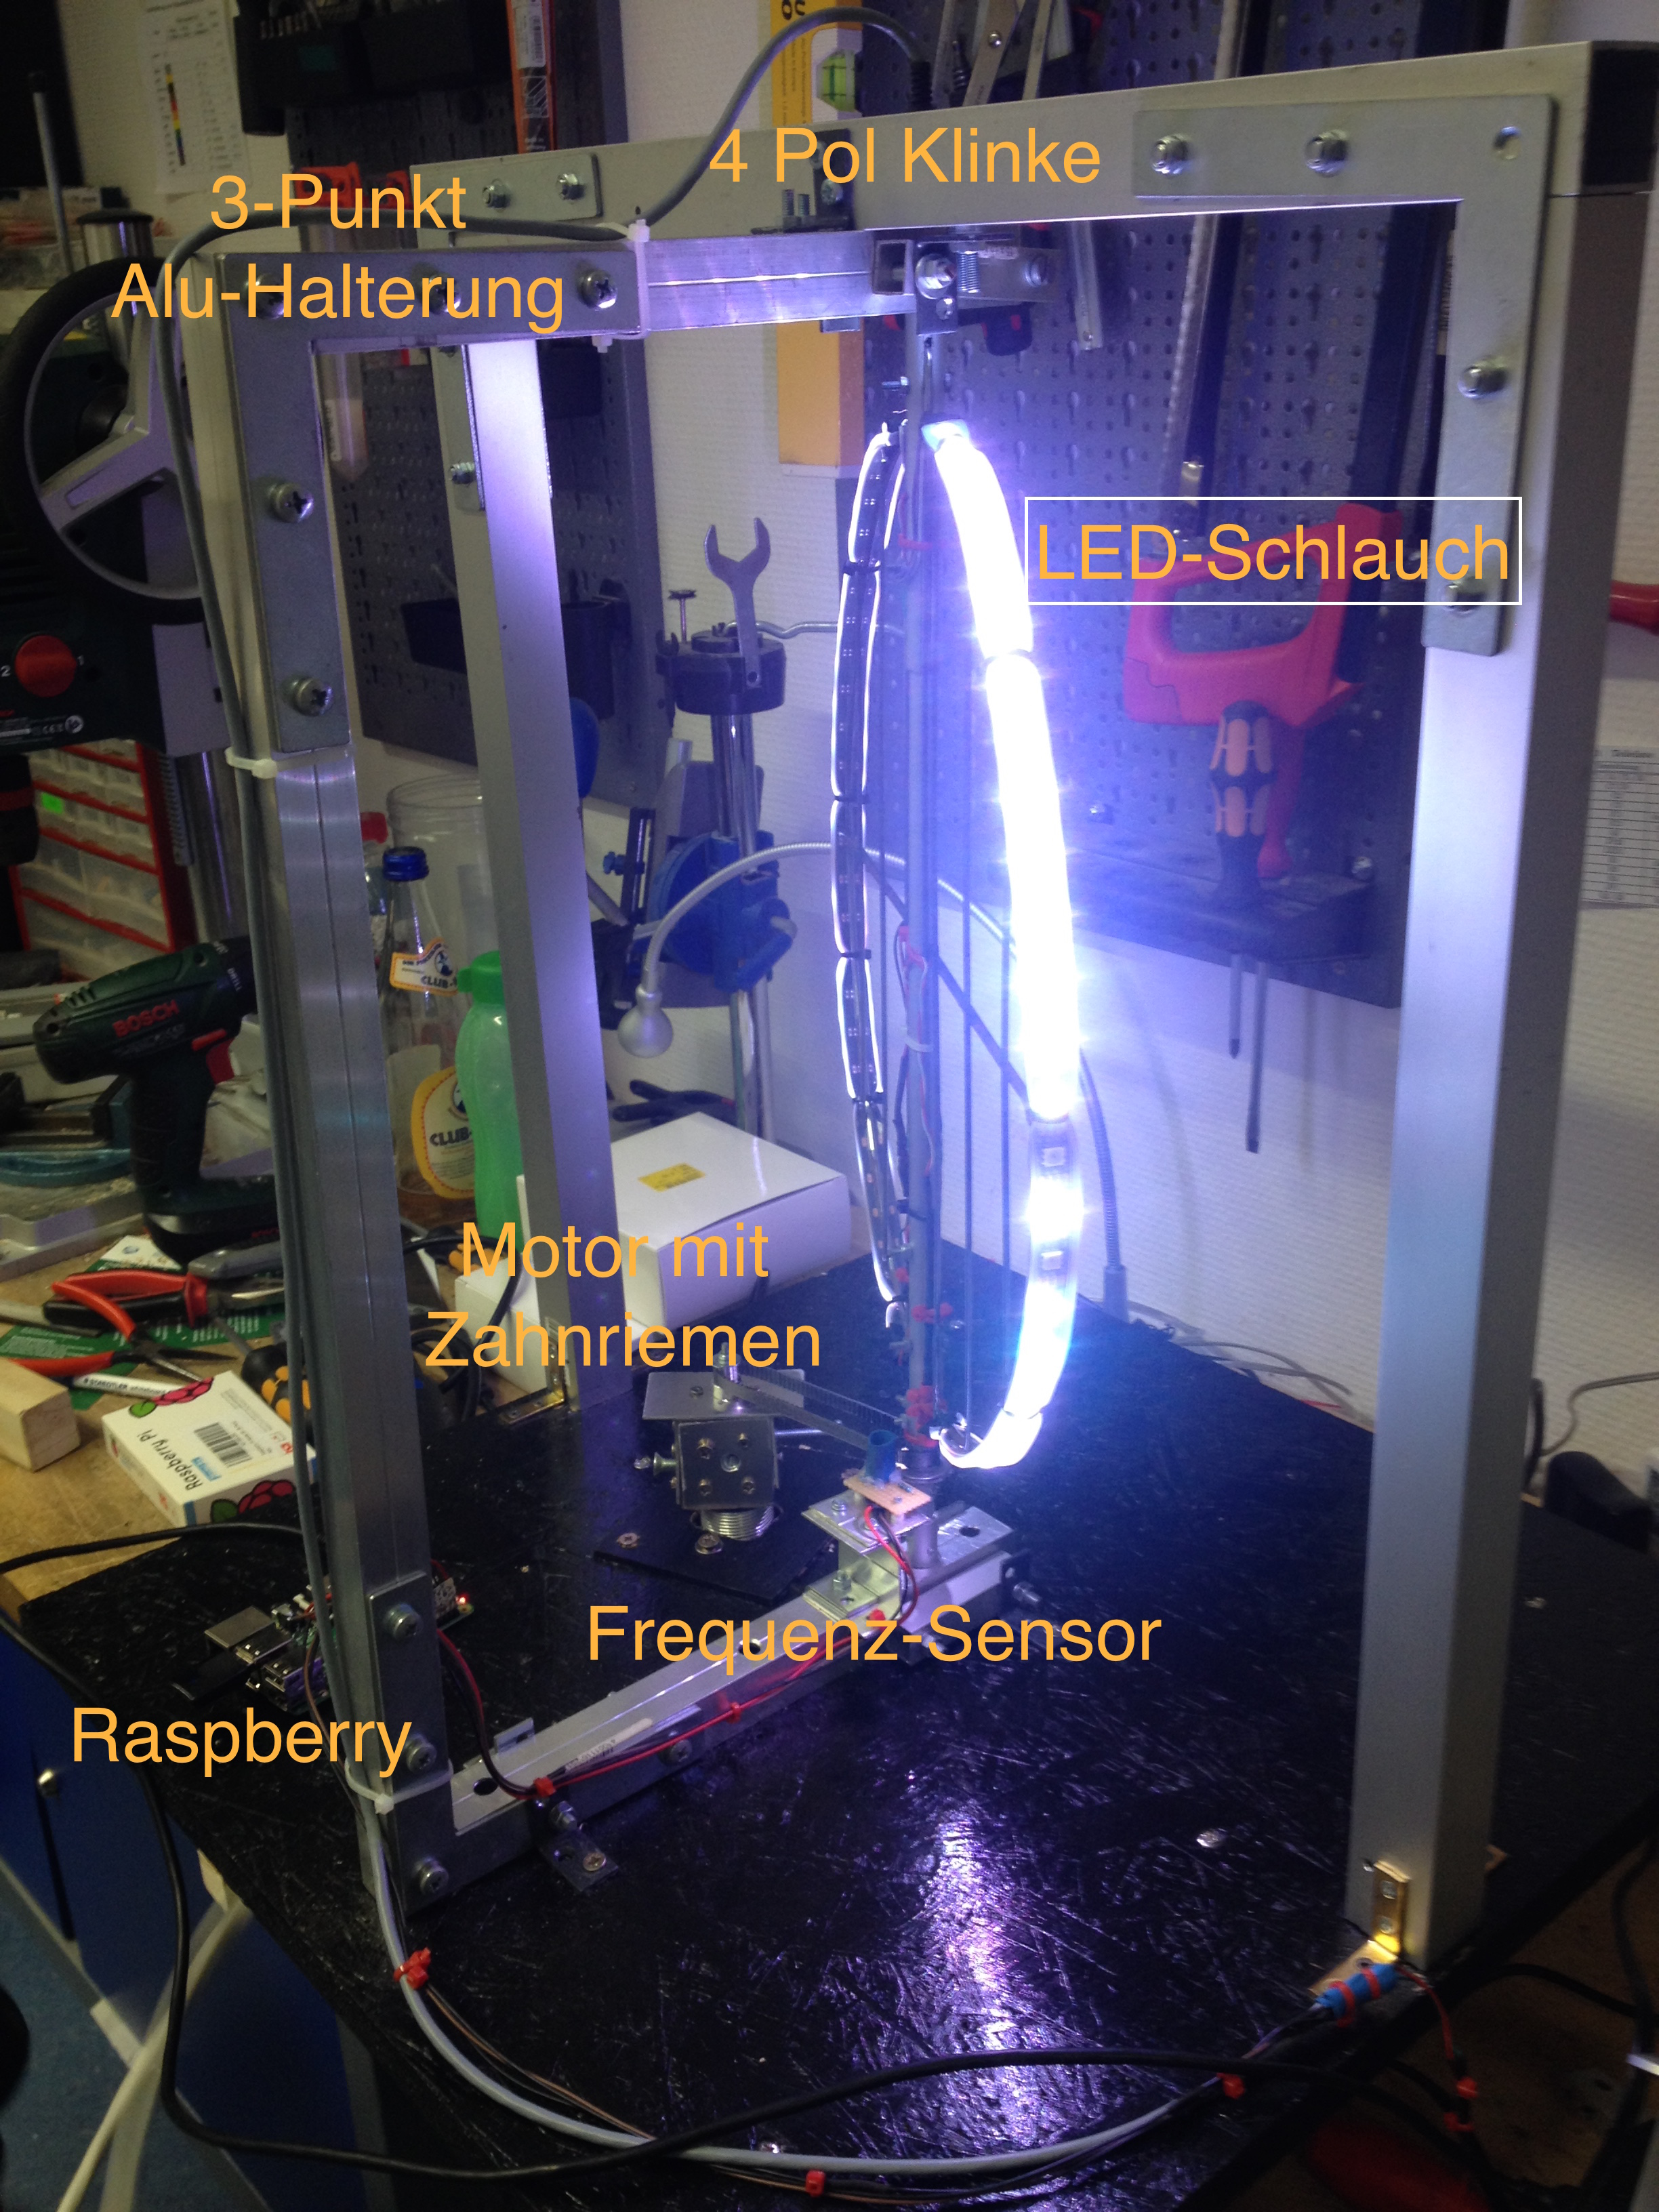
\includegraphics[height=1.19\textheight]{Plots/Komponenten.jpg}
\end{figure}
\end{frame}

\begin{frame}{}
\vspace*{-.5cm}
\begin{figure}
\center
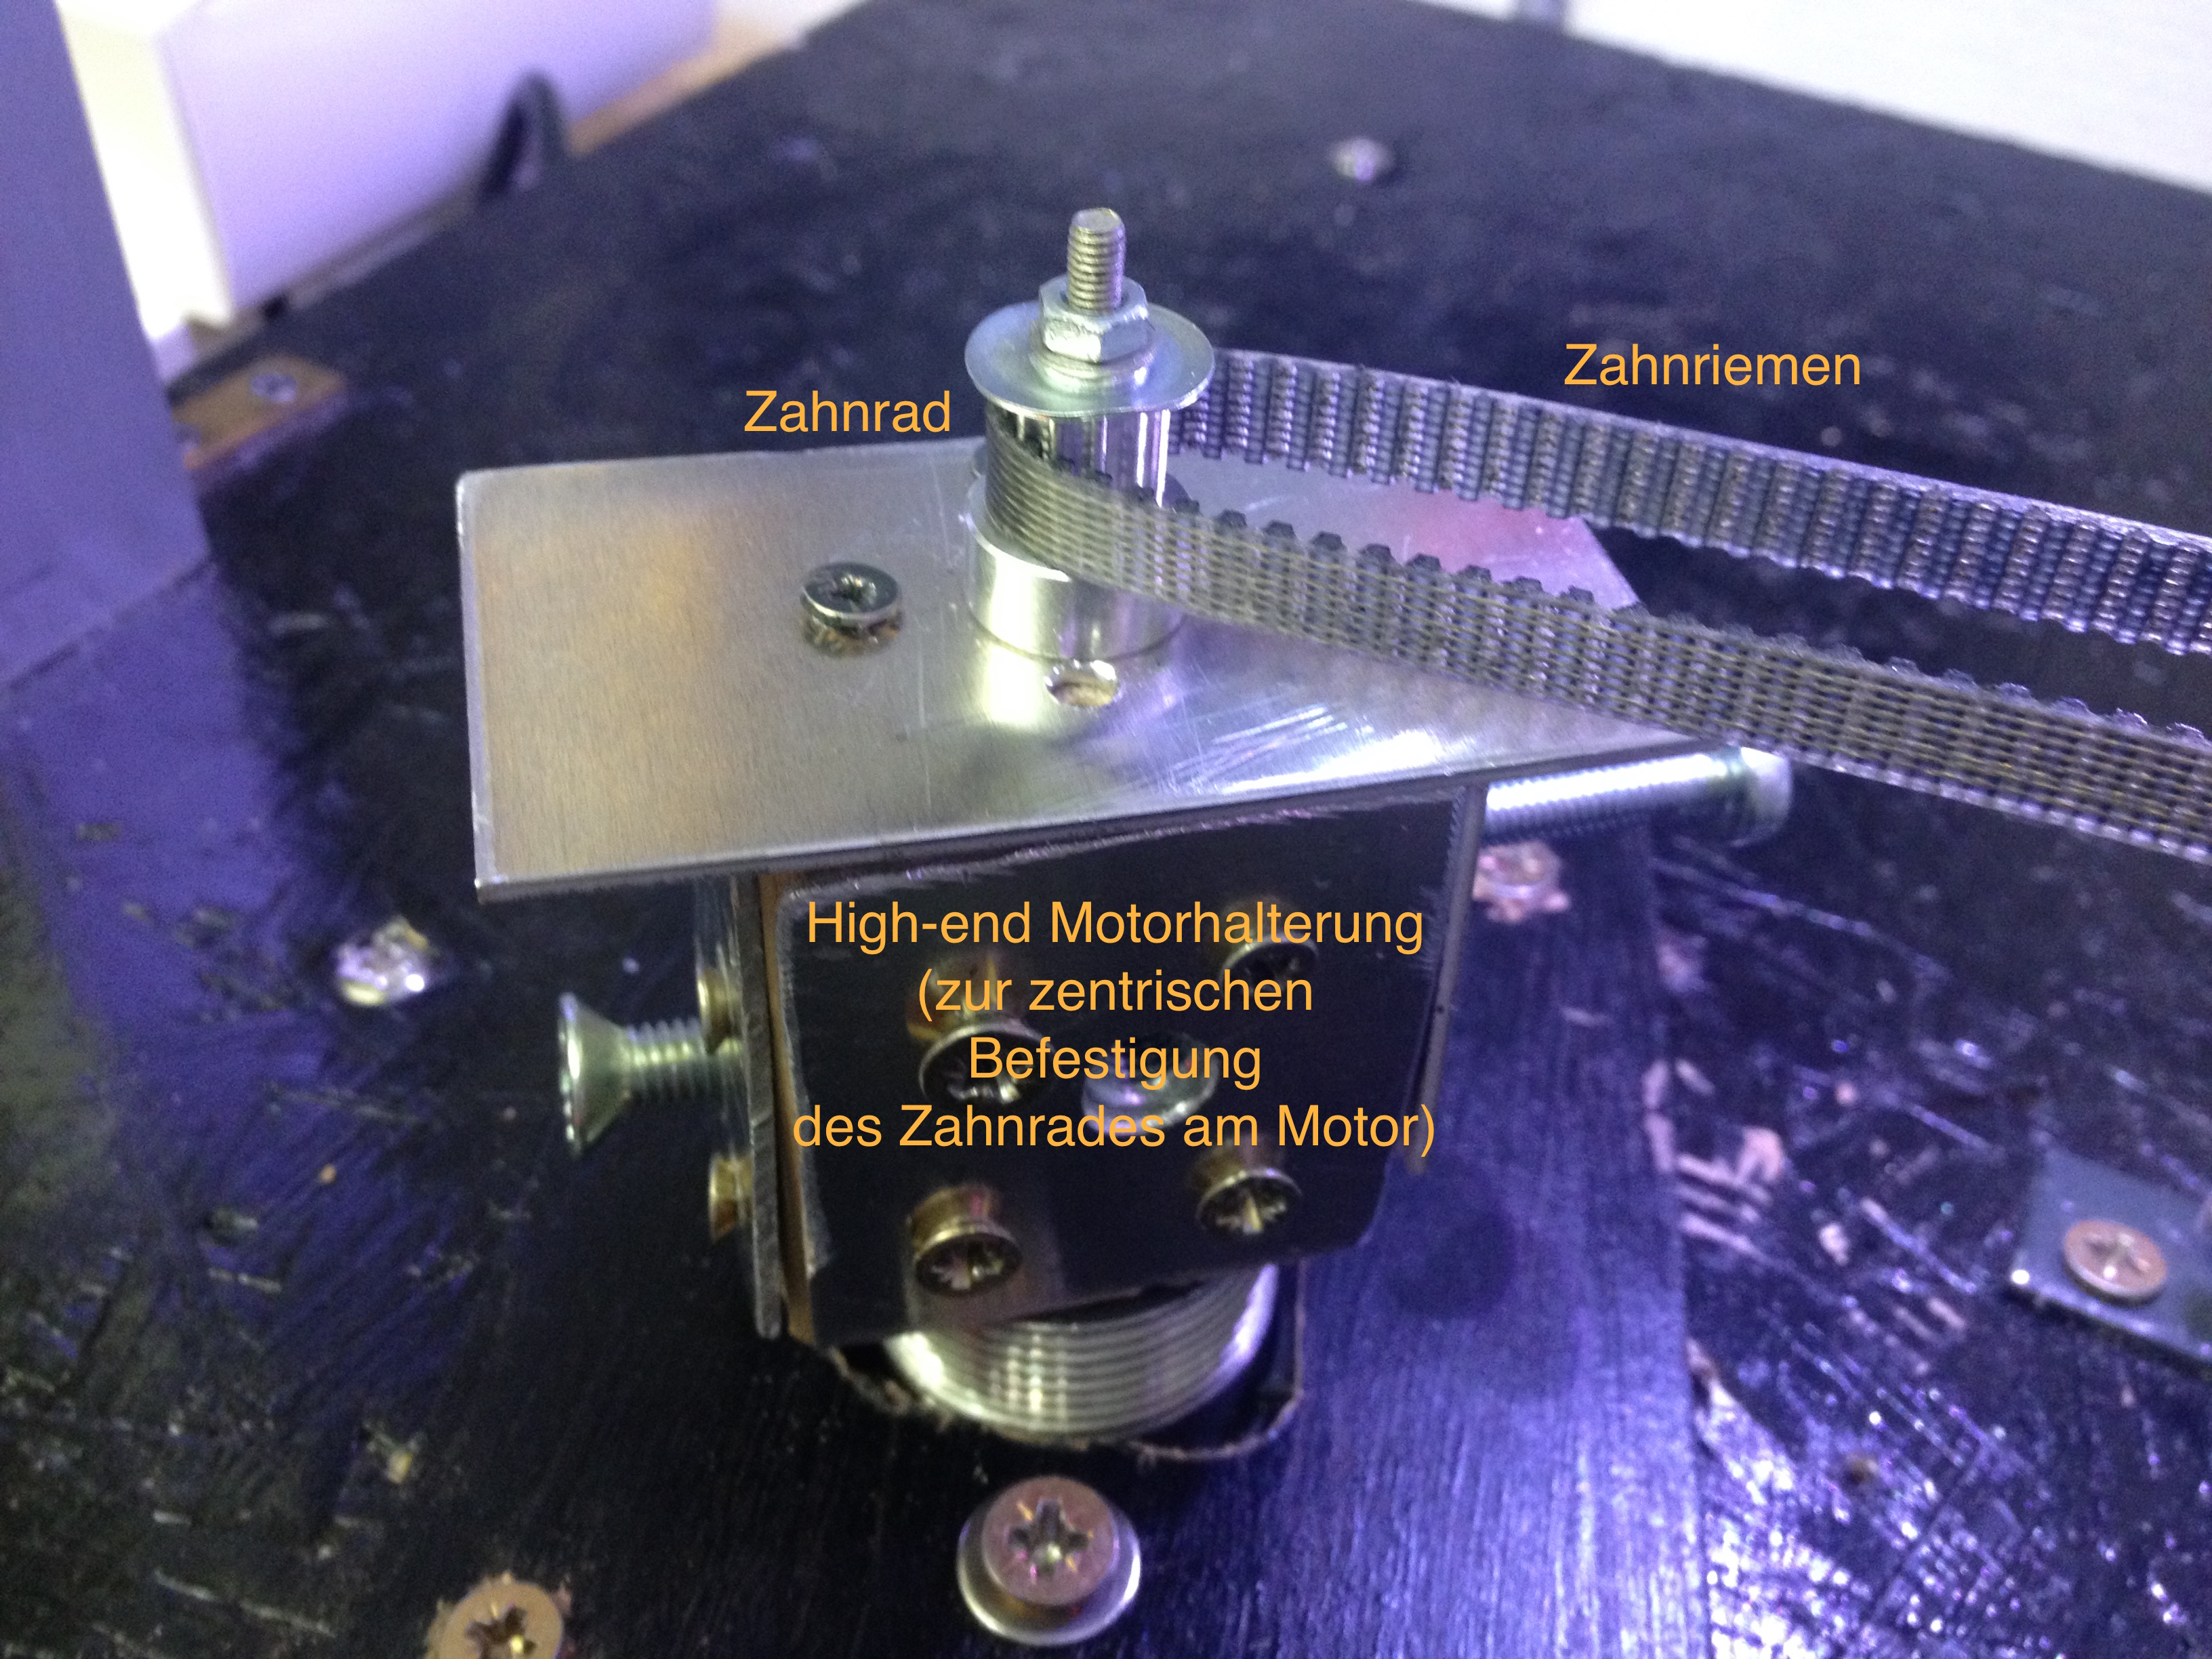
\includegraphics[height=\textheight]{Plots/Motor_oben}
\end{figure}
\end{frame}

\begin{frame}{}
\vspace*{-.5cm}
\begin{figure}
\center
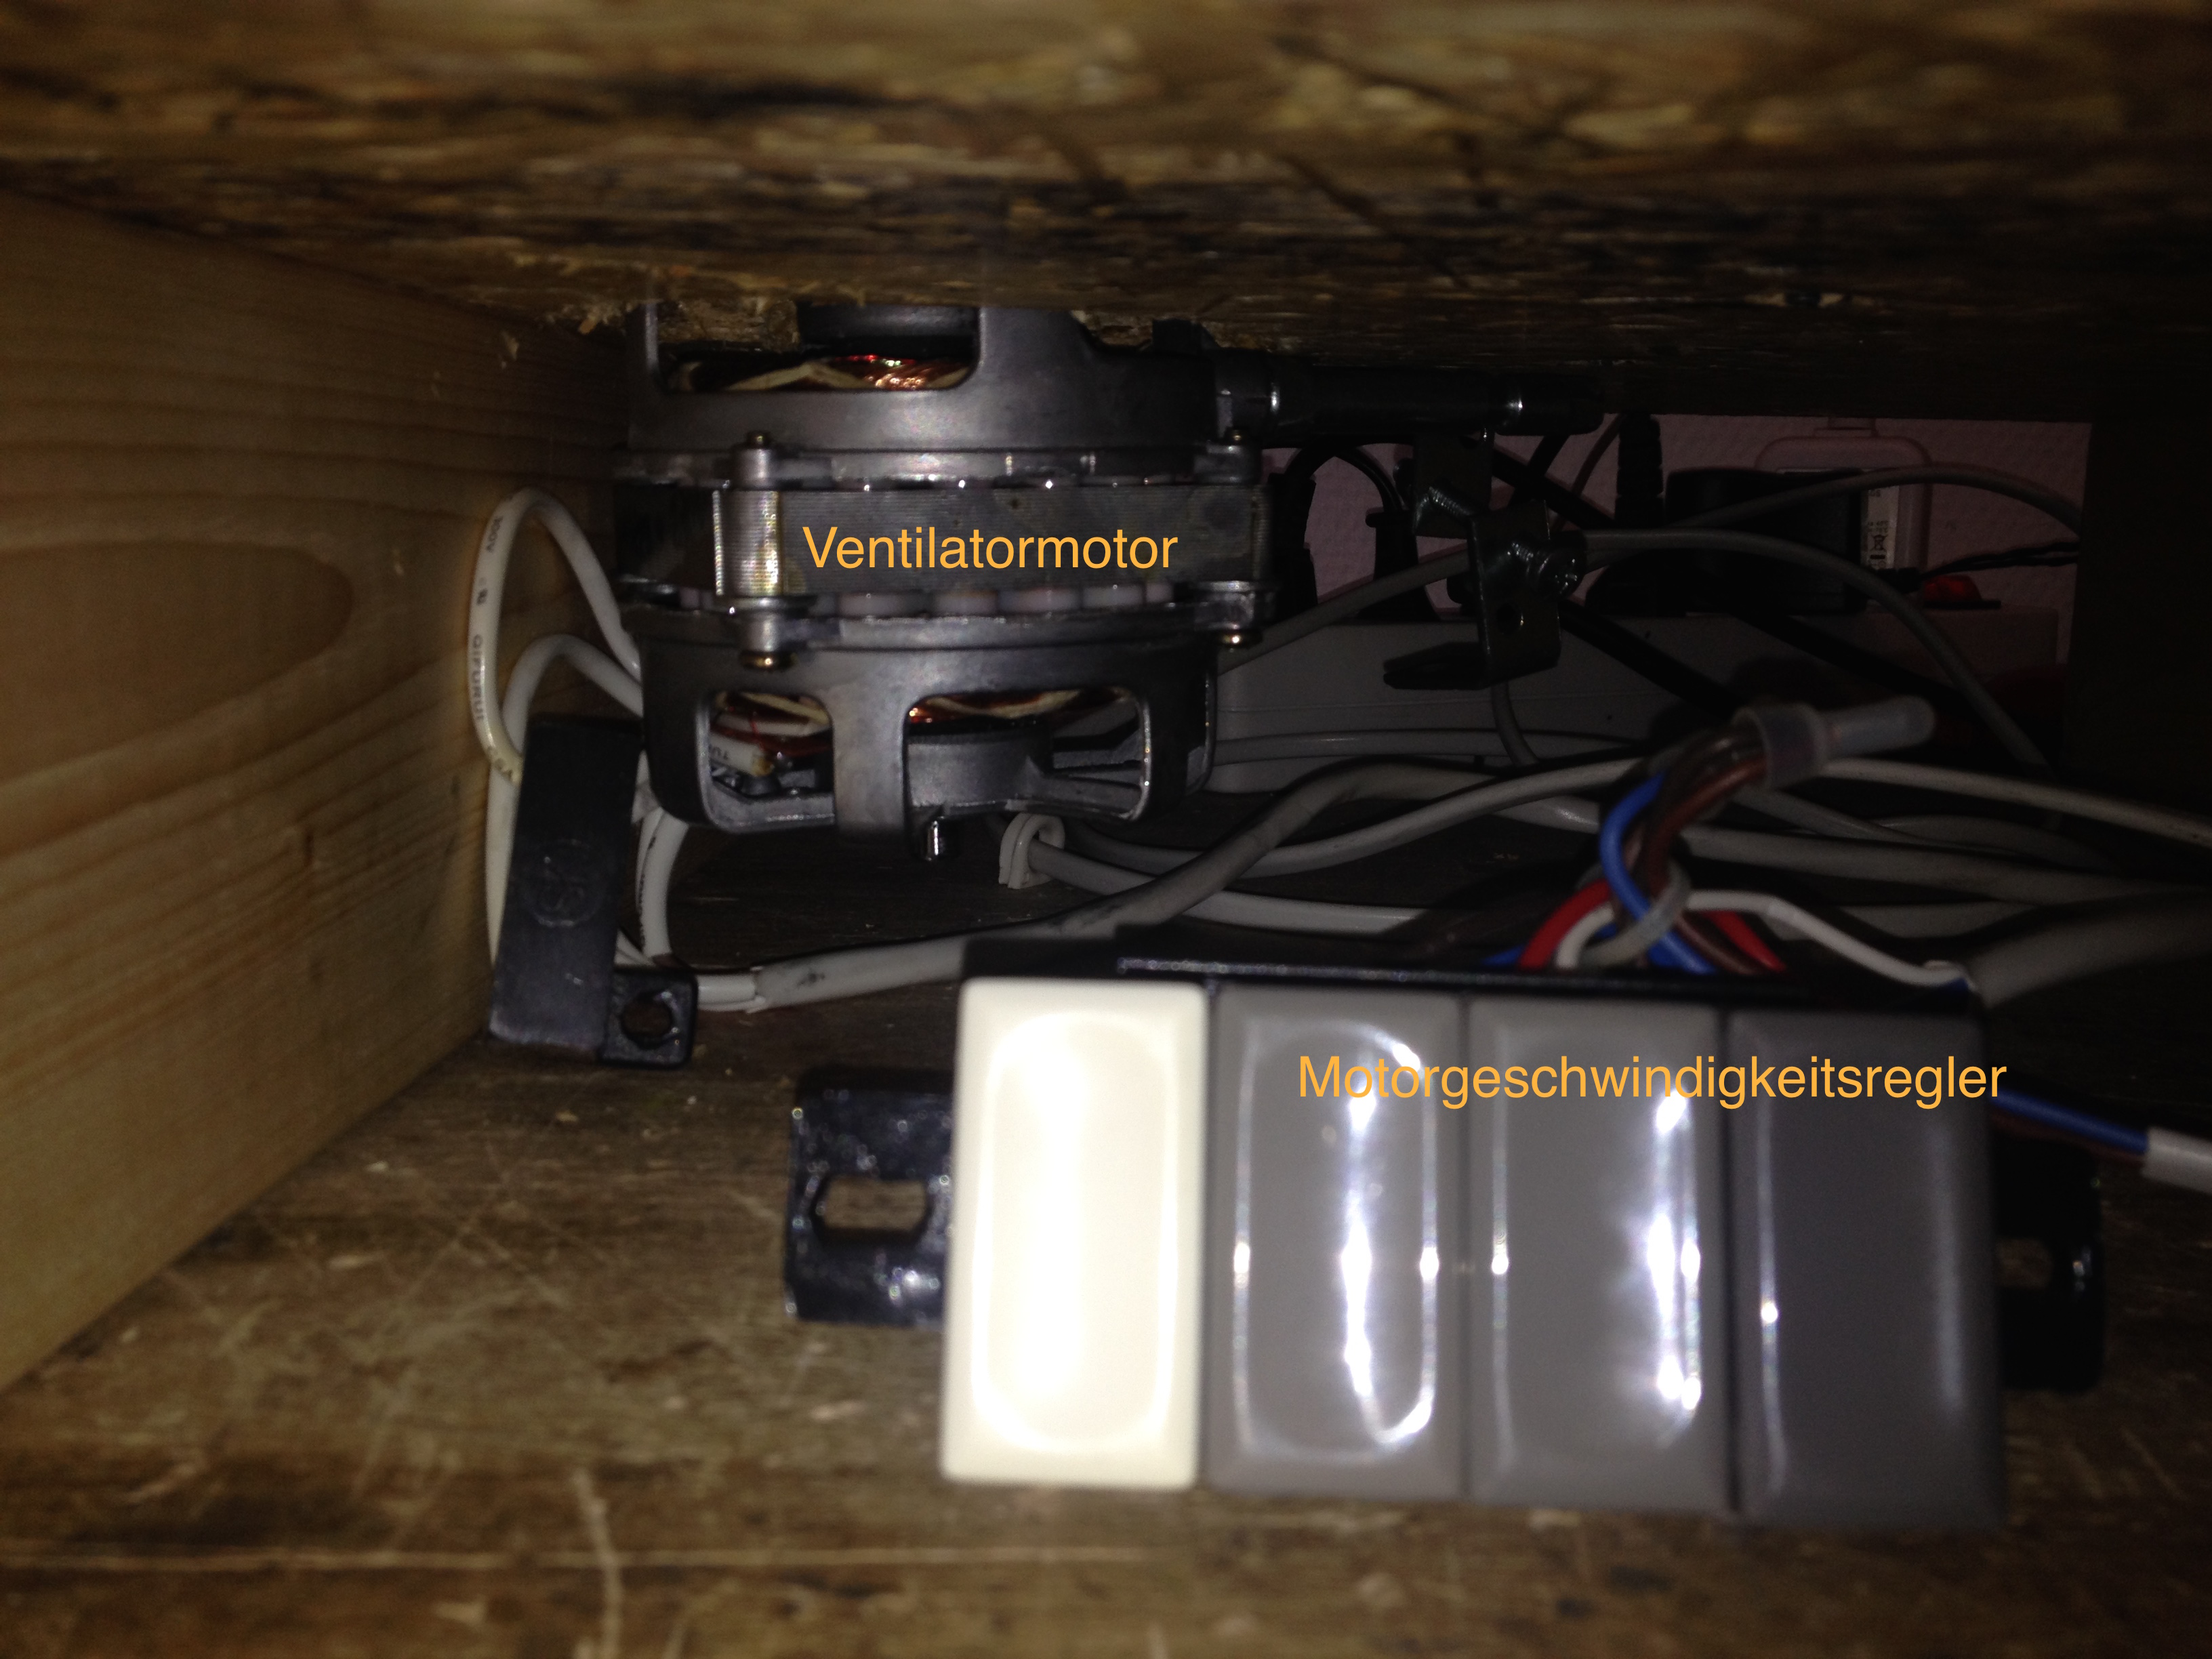
\includegraphics[height=\textheight]{Plots/Motor}
\end{figure}
\end{frame}

\begin{frame}{}
\vspace*{-.5cm}
\begin{figure}
\hspace*{-.5cm}
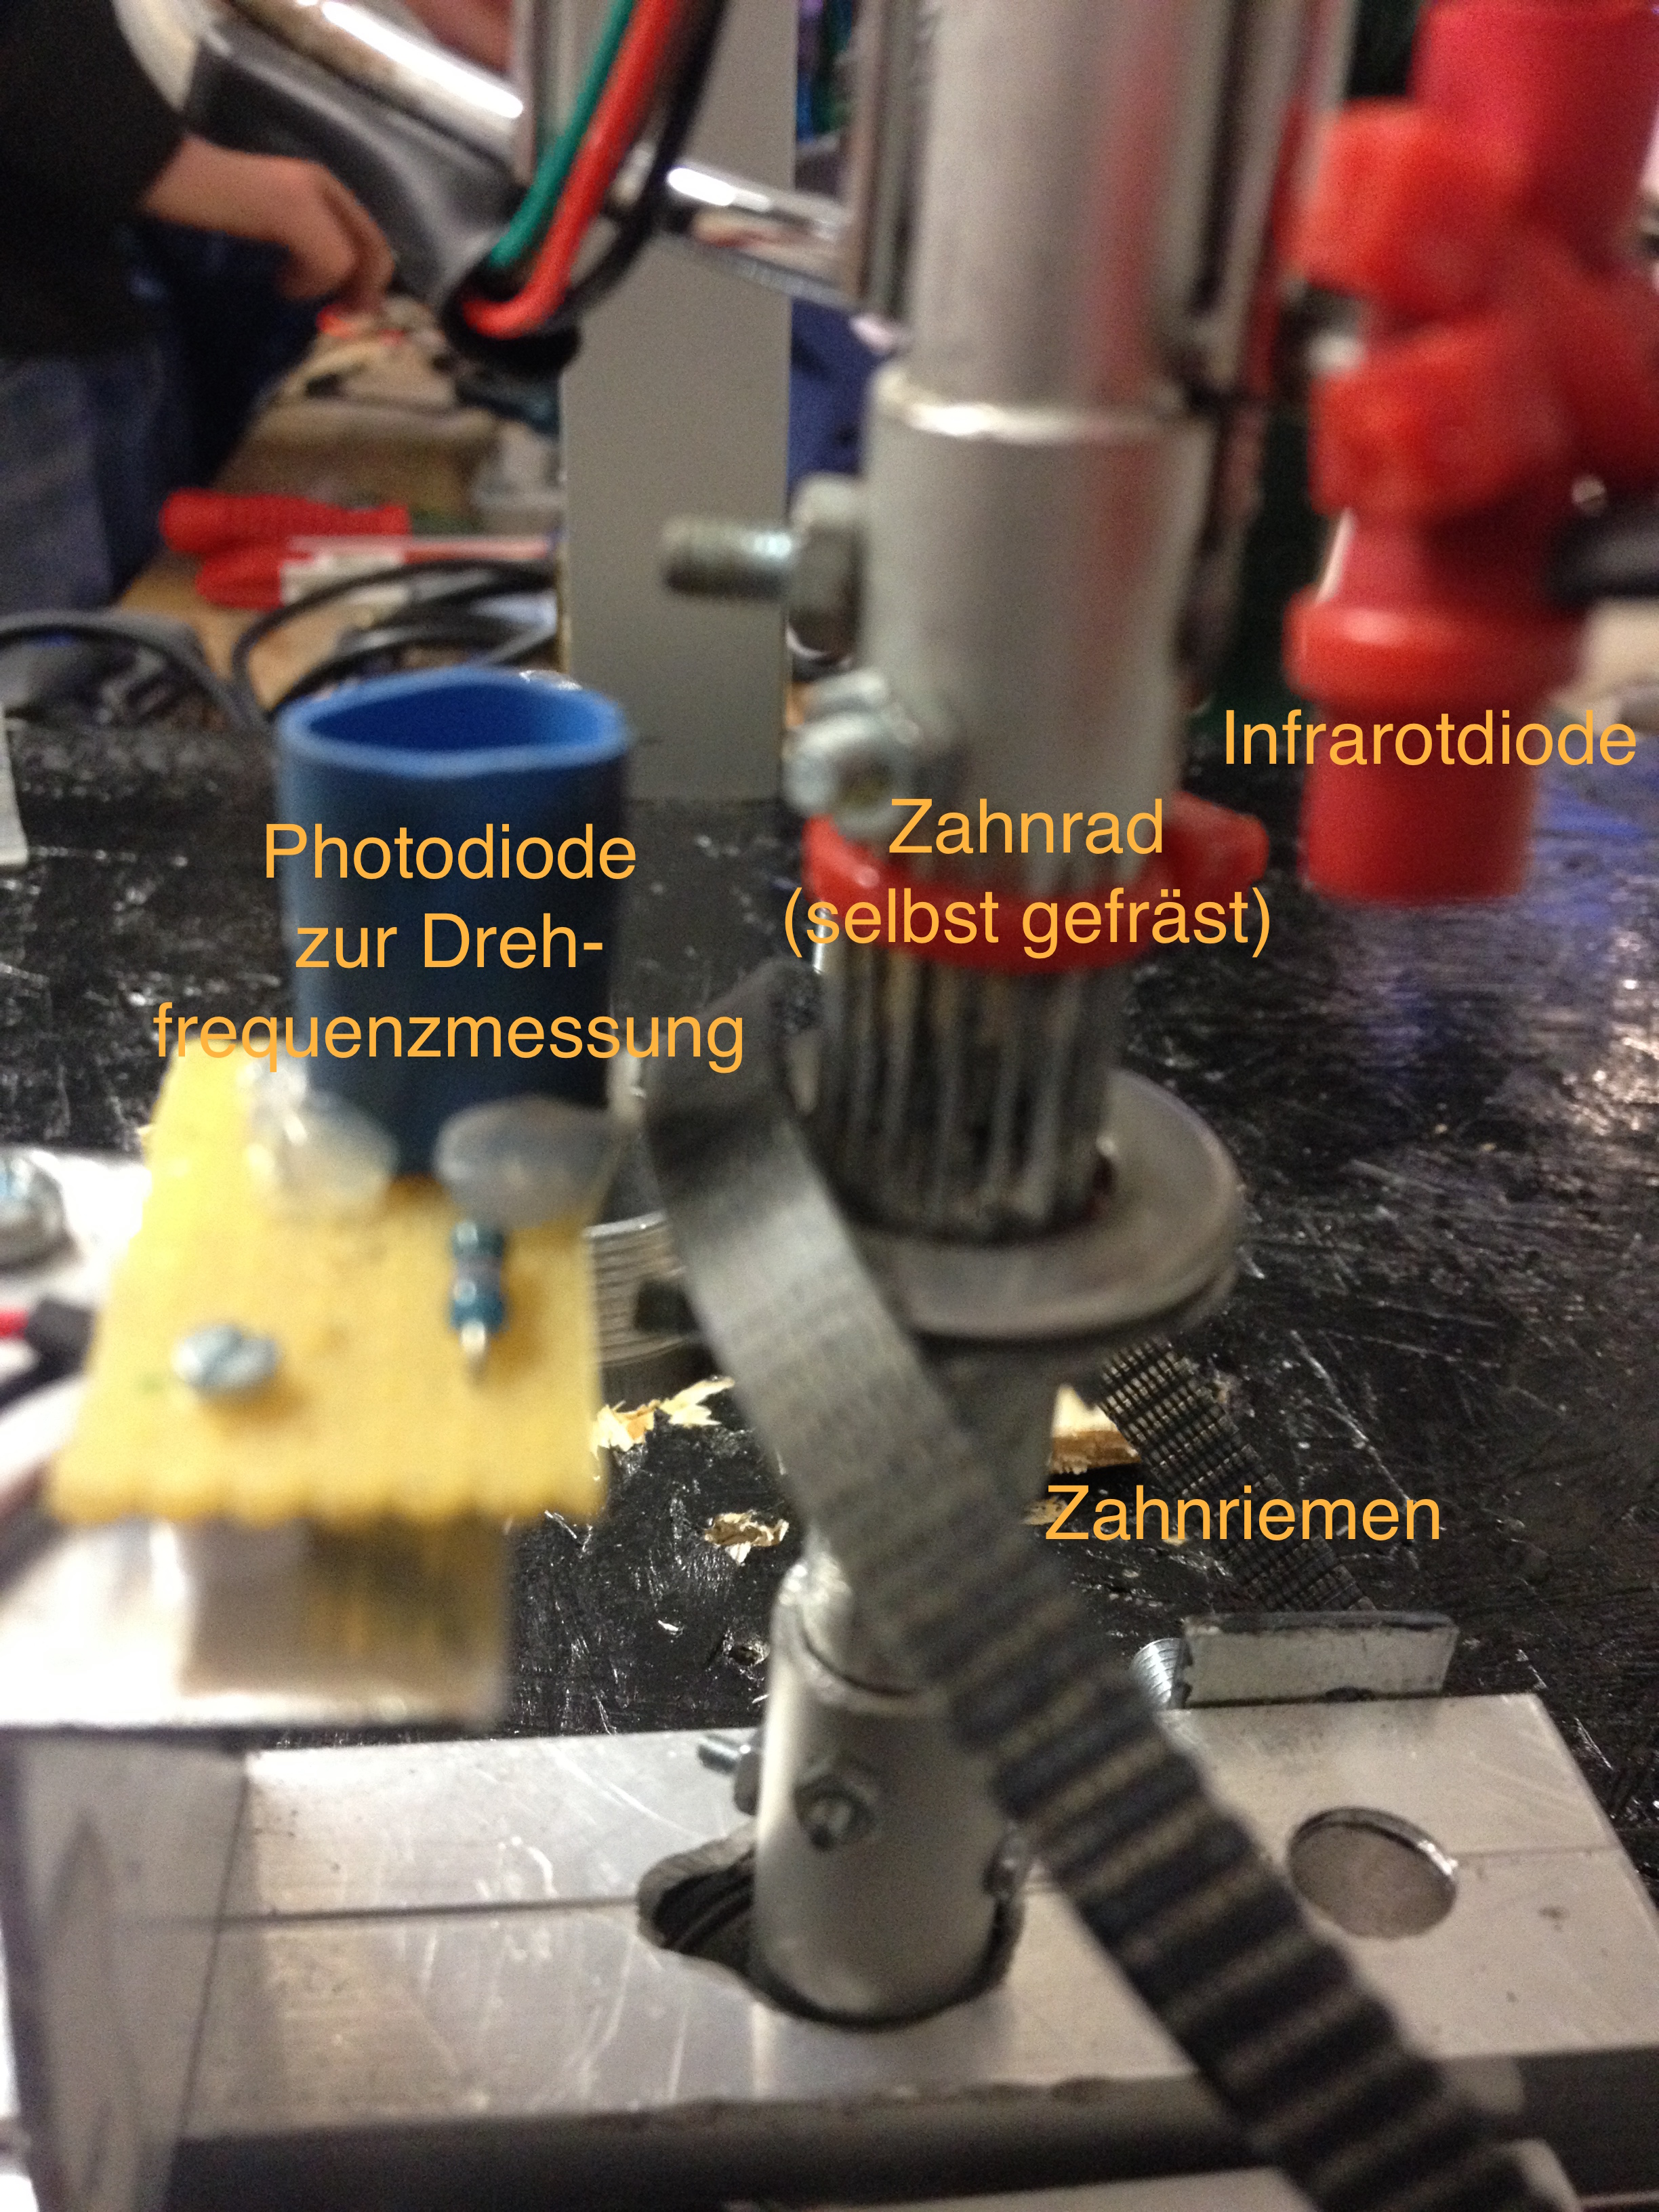
\includegraphics[width=.525\textwidth]{Plots/Zahnriemen}
\hspace*{.1cm}
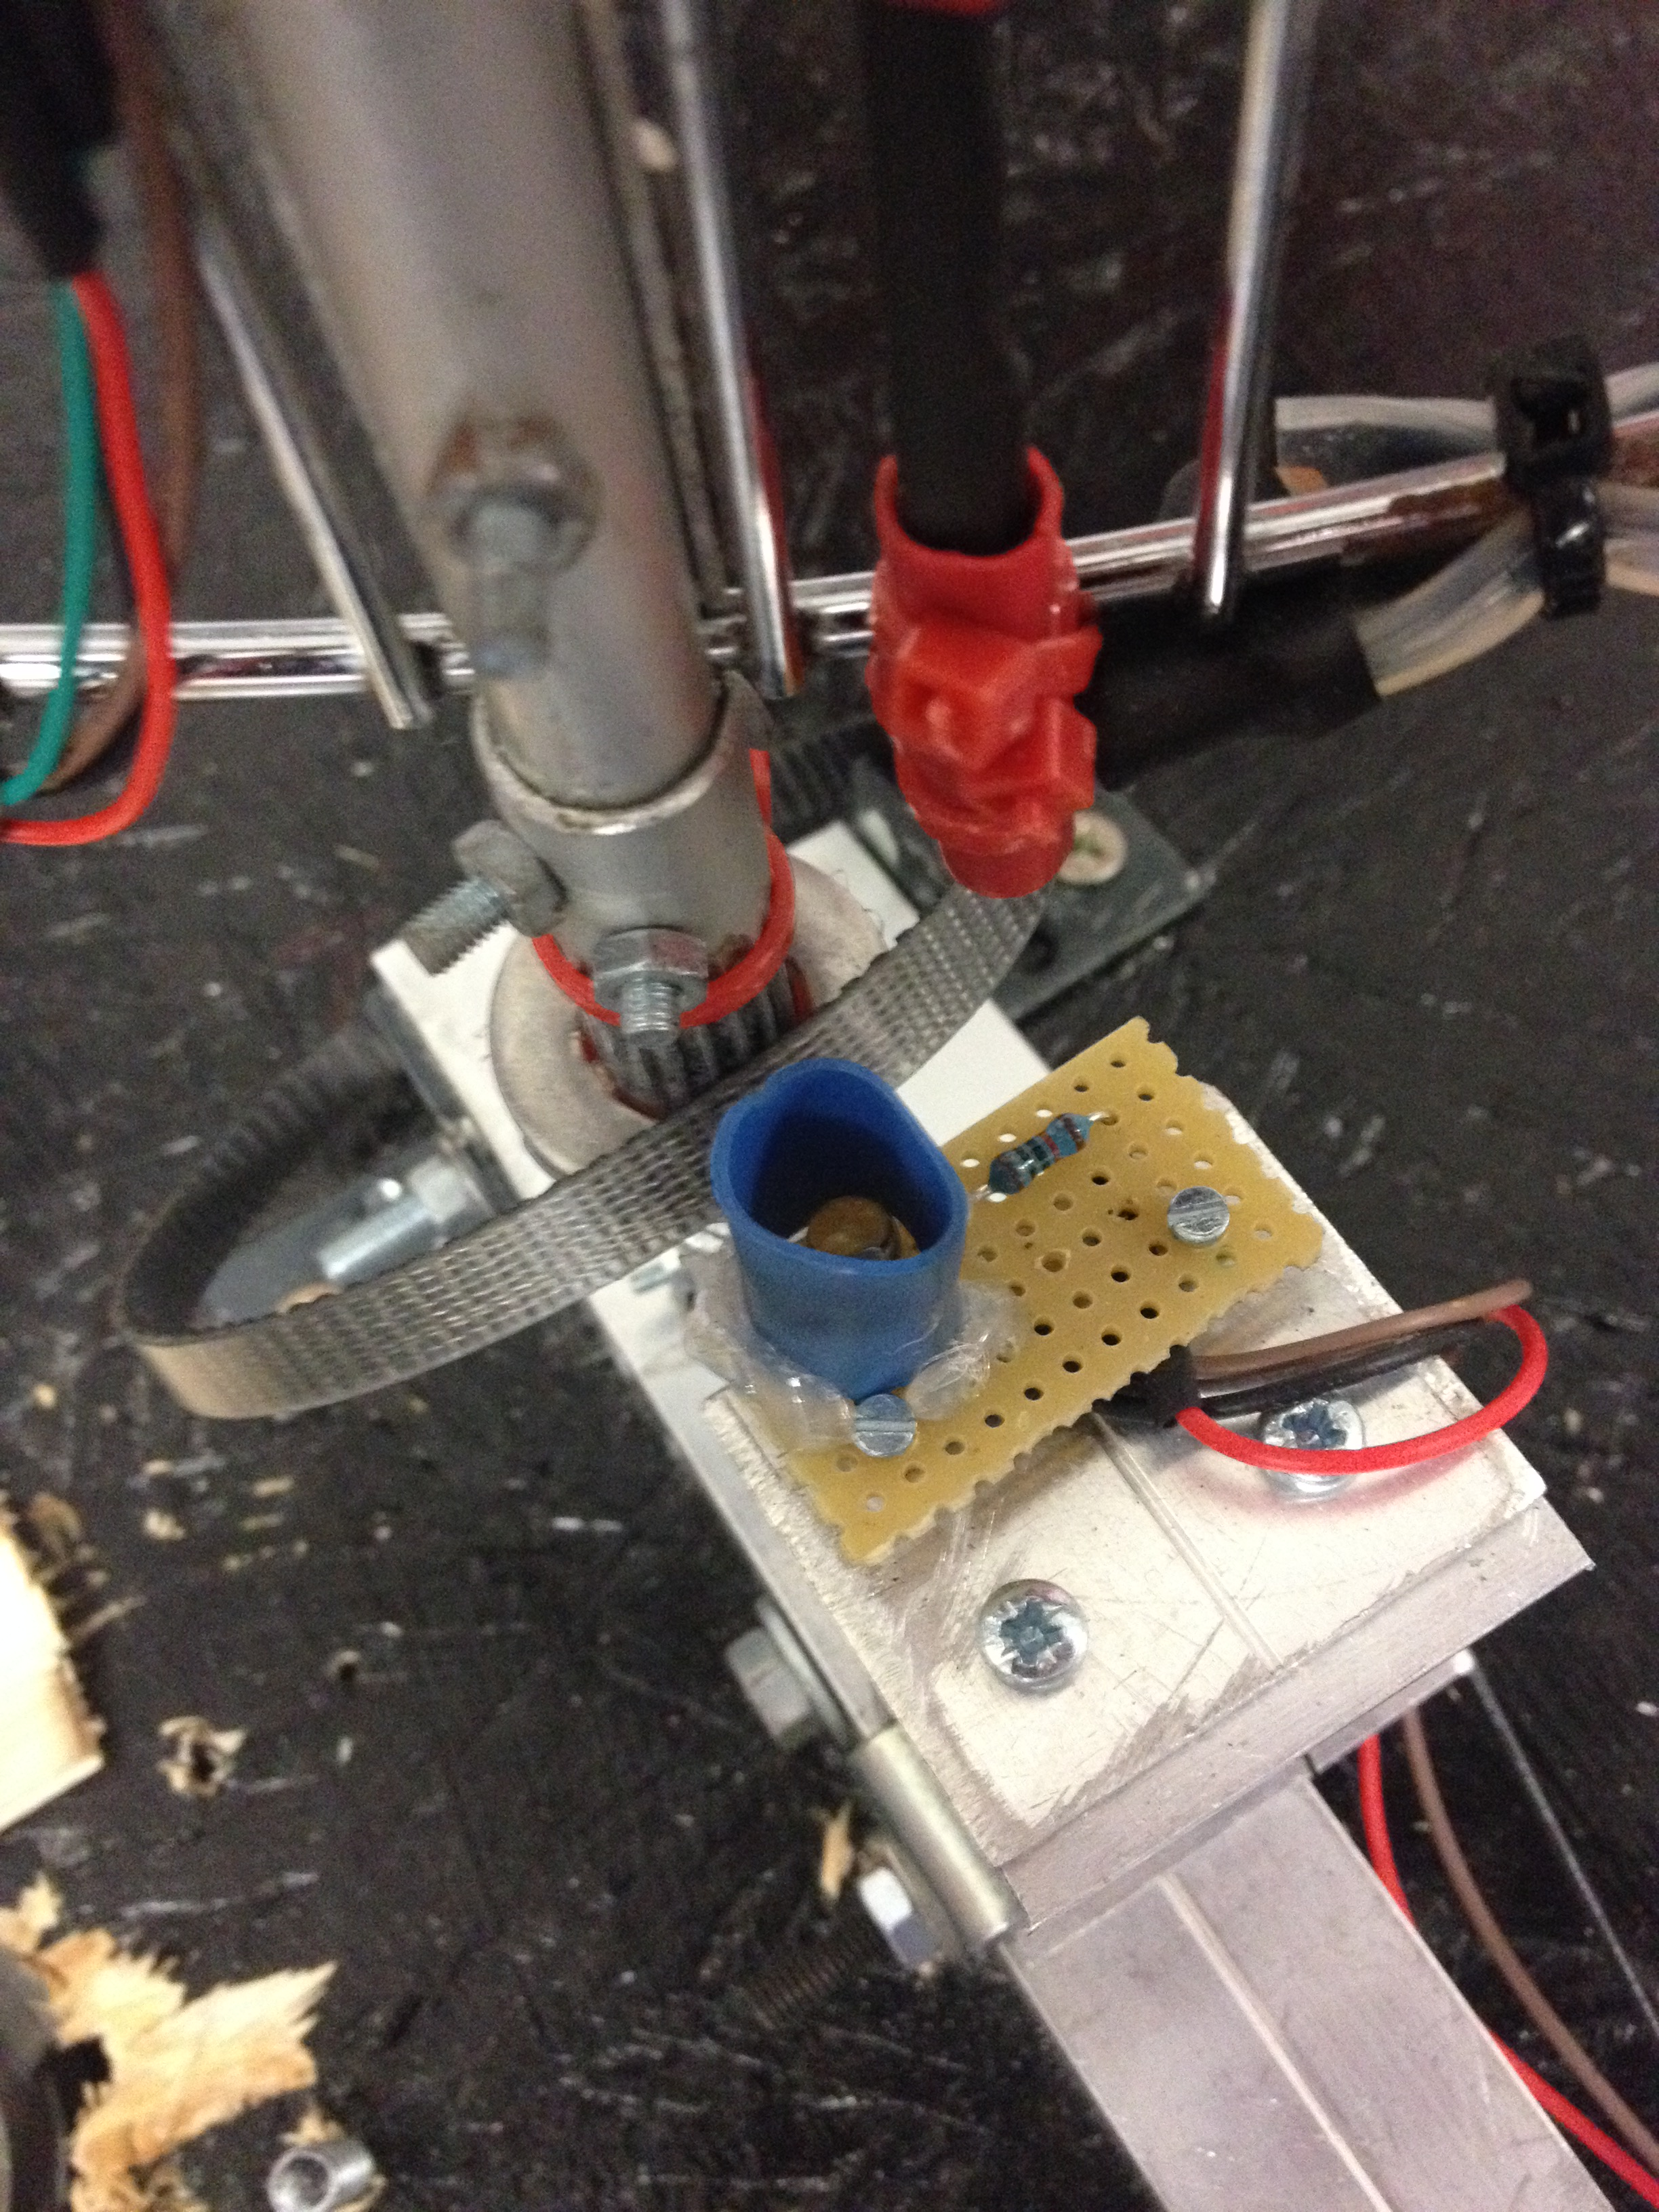
\includegraphics[width=.525\textwidth]{Plots/Photodiode}
\end{figure}
\end{frame}

\begin{frame}{}
\vspace*{-.5cm}
\begin{figure}
\center
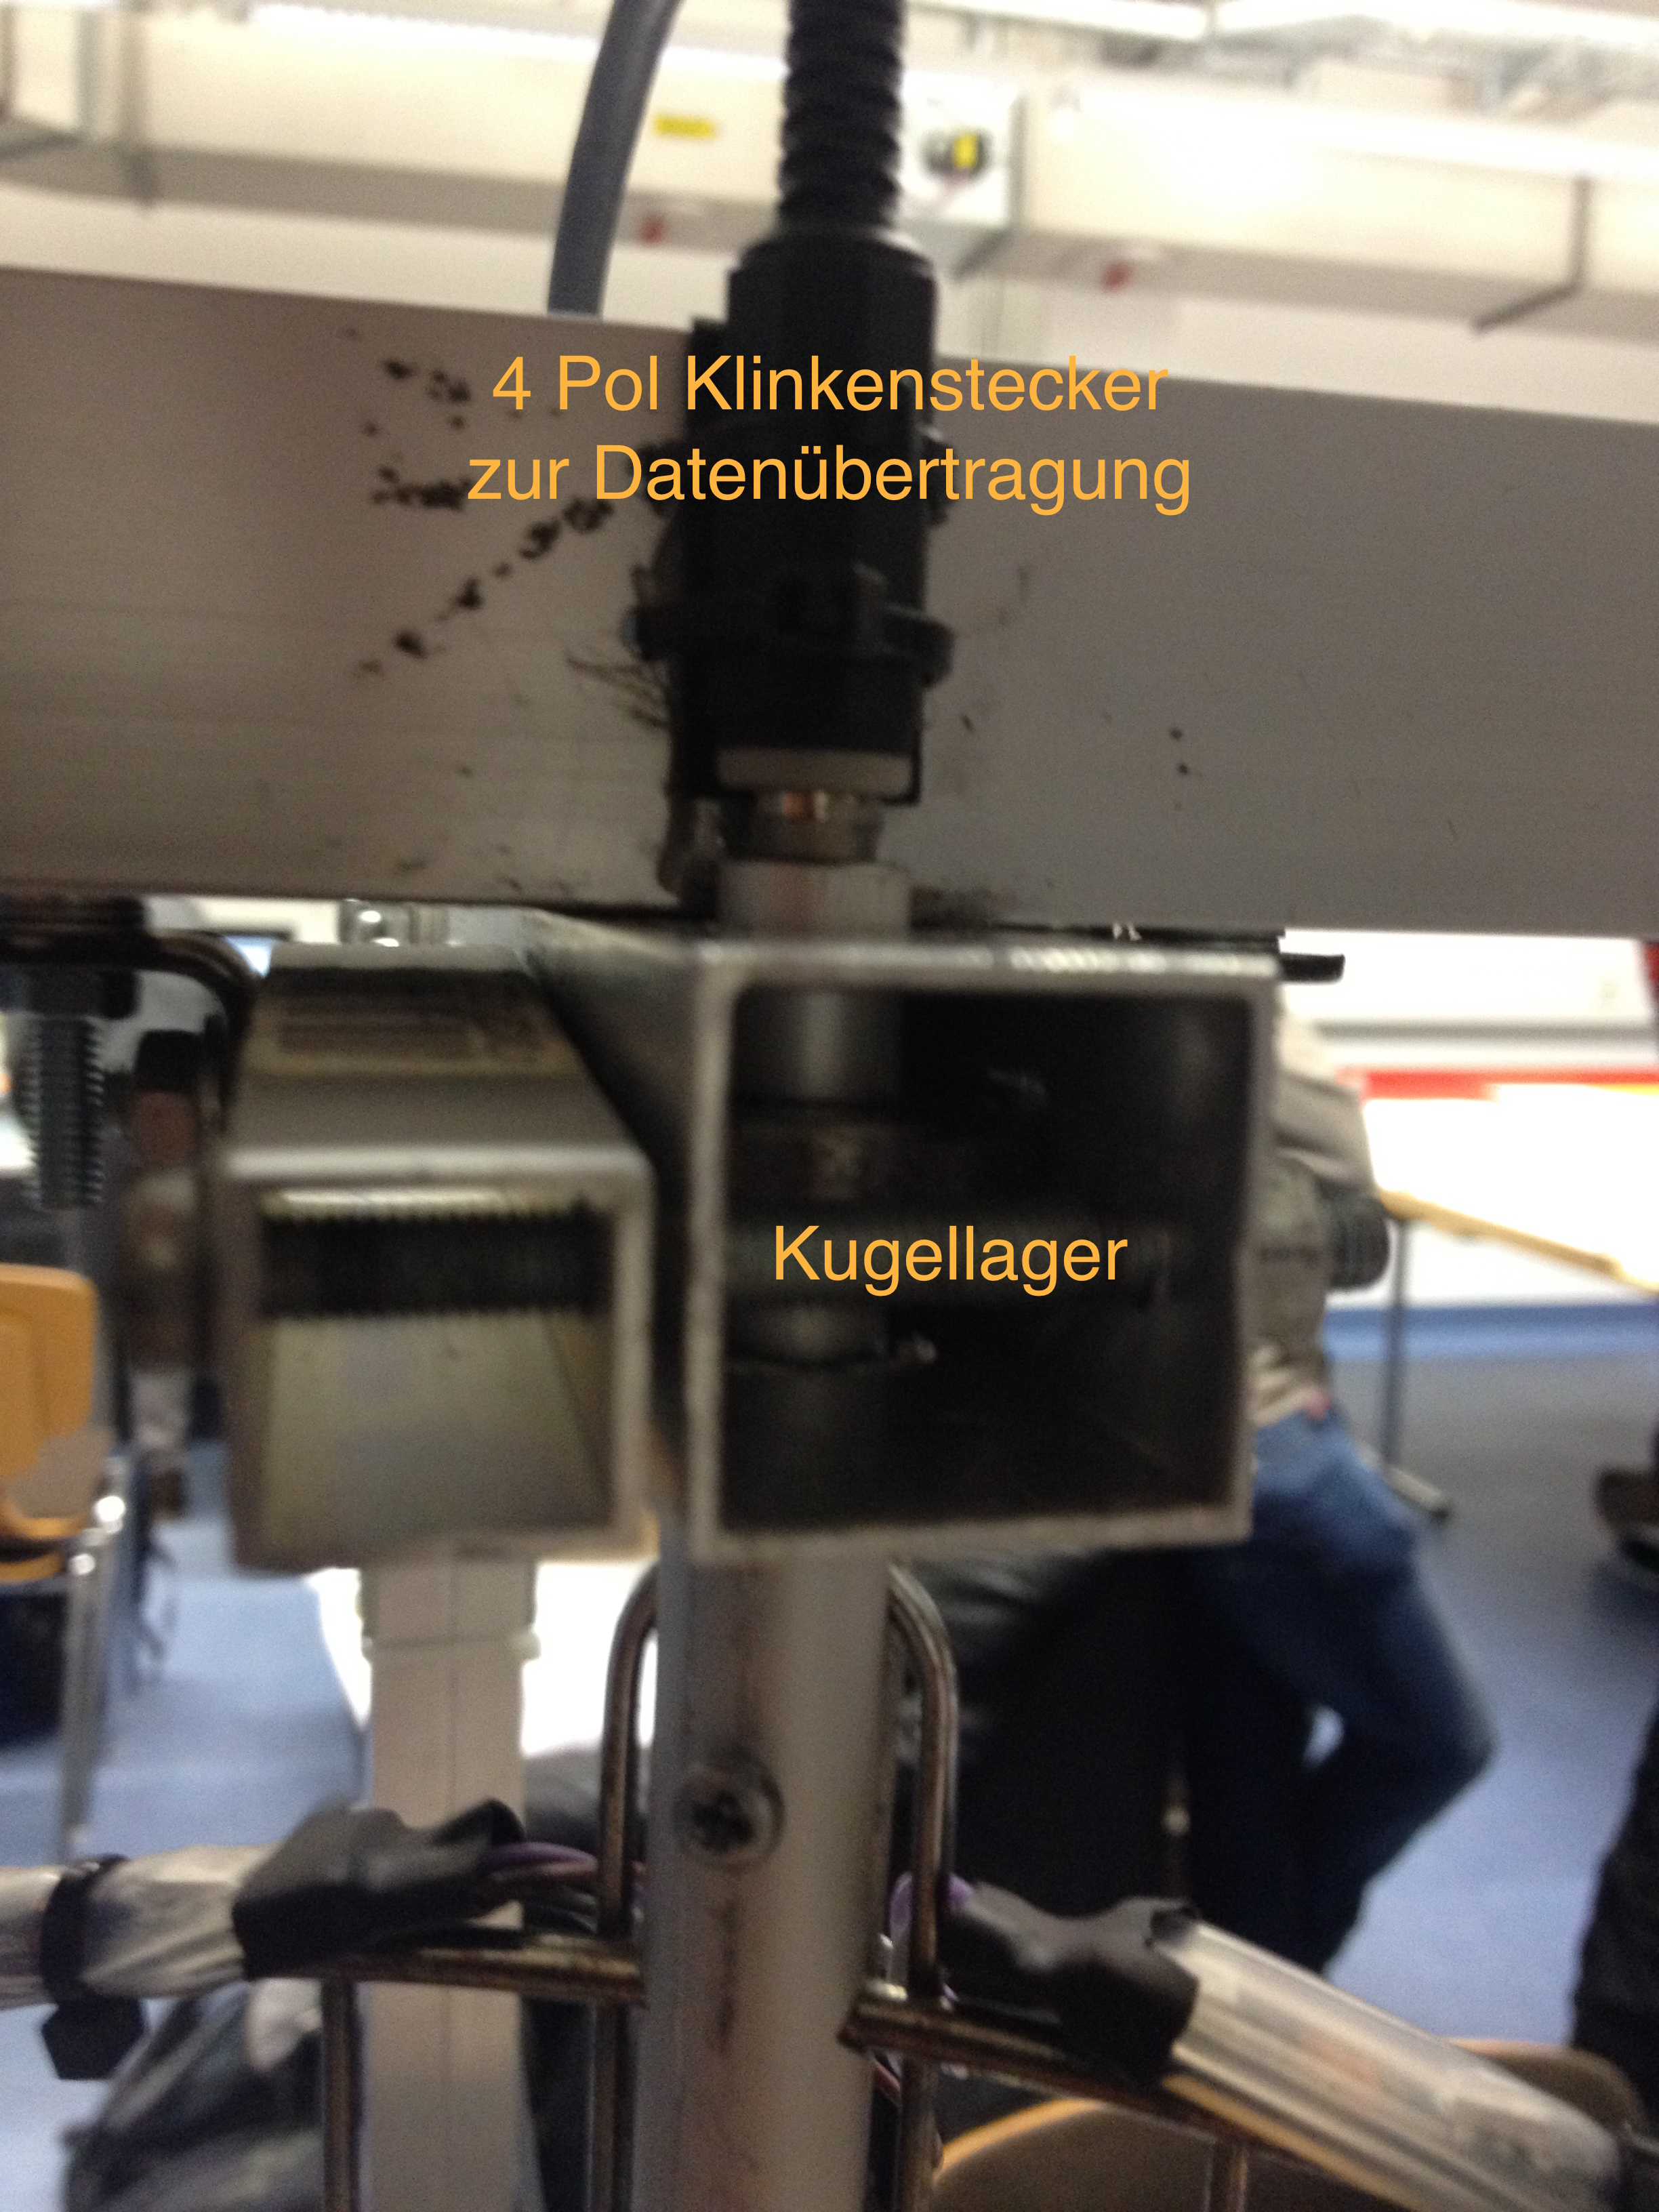
\includegraphics[height=\textheight]{Plots/Klinke}
\end{figure}
\end{frame}

\begin{frame}{Features}
\begin{figure}
\center
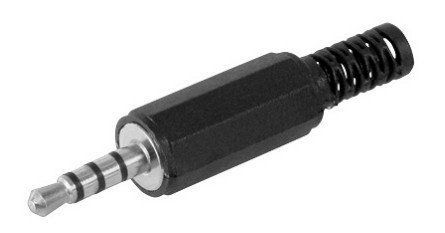
\includegraphics[height=0.25\textheight]{Plots/Klinke2}
\end{figure}
\begin{exampleblock}{}
Datenübertragung über 4 Pol Klinke (axial gelagert)
\\\ \\
\begin{itemize}
\item Idee: Nur der LED-Schlauch soll rotieren
\item LED Schlauch benötigt 4 Anschlüsse: VCC, GND, DATA, CLOCK 
\item Übertragung der Daten auf rotierende Elemente via 4 Pol Klinke
\end{itemize}
\end{exampleblock}
\end{frame}

\section{Realisierung und Code}

\begin{frame}{Datenaufbereitung}
Zur optimalen Ausnutzung des 60 LED-Schlauchs:\\
Invertierung und Schachtelung der Zeilen!\\
\ \\
Mapping:\\
LED \ 0 \rightarrow\ Zeile 58\qquad\qquad\qquad LED 30 \rightarrow\ Zeile \ 1\\
LED \ 1 \rightarrow\ Zeile 56\qquad\qquad\qquad LED 31 \rightarrow\ Zeile \ 3\\
LED \ 2 \rightarrow\ Zeile 54\qquad\qquad\qquad LED 32 \rightarrow\ Zeile \ 5\\
...\qquad\qquad\qquad\qquad\qquad\qquad\ \ ...\\
LED 29 \rightarrow\ Zeile \ 0\qquad\qquad\qquad LED 59 \rightarrow\ Zeile 59\\
\ \\
\Rightarrow\ Formel:\\
LEDs 0 - 29: i \rightarrow\ $60-2\times(1+i)$\\
LEDs 30-59:  i \rightarrow\ $1+2\times(i-30)$
\end{frame}

\begin{frame}{Datenaufbereitung (Python)}
%\begin{listings}
%\end{listings}
\lstinputlisting[firstline=25,lastline=42]{pngTOpov_demo.py}
\end{frame}

\begin{frame}{Datenaufbereitung (Python)}
Außerdem: Verschiebung der Spalten der ungeraden Zeilen!\\
\begin{itemize}
\item gerade Zeilen: unverändert.
\item ungerade Zeilen:
\begin{itemize}
\item Spalte \ 1-29 \rightarrow\ Spalte 30-59
\item Spalte 31-59 \rightarrow\ Spalte \ 0-29
\end{itemize}
\end{itemize}

%\begin{listings}
%\end{listings}
\lstinputlisting[firstline=47,lastline=57]{pngTOpov_demo.py}
\end{frame}

\begin{frame}{Ansteuerung und Datenübertragung}
Jede LED benötigt 4 bytes: (0, blau, grün, rot)\\
\Rightarrow\ Schlauch wird durch Liste von $4\times60=240$ bytes gesteuert.\\
\ \\
Die Umsetzung wird durch die Bibliothek \emph{dotstart} von \emph{Adafruit\_DotStar} mittels Clock- und Data-PINs (GPIO) realisiert.\\
\end{frame}

\begin{frame}{Ansteuerung und Datenübertragung}{}
{\bf Wichtig:} Exakt richtiges Timing!\\
\ \\
\sim7 Umdrehungen pro Sekunde $=60$ Spalten \Rightarrow\ \sim0.0024s pro Spalte\\
\rightarrow\ kleine Abweichung führt zu Verschiebung im Bild!\\
\ \\
{\bf Lösung zur Stabiliesierung:}\\
\begin{itemize}
\item Infrarot-LED misst Rotationsfrequenz
\item Script überprüft verstrichene Zeit im Code
\item \Rightarrow\ angepasste Verzögerung zwischen einzelnen Spalten
\end{itemize}
\end{frame}

\begin{frame}{Datenübertragung (Python)}
%\begin{listings}
%\end{listings}
\lstinputlisting[firstline=106,lastline=125]{show_pov_demo.py}
\end{frame}

\section{Probleme}

\begin{frame}{Probleme}
\begin{itemize}
\item Probleme mit diversen Motoren
\item[] \rightarrow\ diverse Konzepte ausprobiert
\item Datenübertragung (Abrieb des Klinkensteckers; fehleranfällig)
\item Lagerung des Kreises
\item zentrische Lagerung der gesamten Konstruktion
\item exakte Anpassung des Skripts an Rotationsfrequenz
\item zerstörter LED-Schlauch
\end{itemize}
\end{frame}

\section{Ausblick}

\begin{frame}{Ausblick}
\begin{itemize}
\item Verbesserung der Bildverarbeitung
\begin{itemize}
\item bewegte Bilder
\item Schrift / Laufschrift
\item Spiele programmieren
\end{itemize}
\item bessere Lagerung
\item besserer Motor
\item höhere Anzahl an Pixel
\end{itemize}
\end{frame}

\begin{frame}
\begin{center}
\textcolor{darkred}{\huge Vielen Dank für Ihre Aufmerksamkeit!}
\end{center}
\end{frame}
